\begin{figure}
  \center
  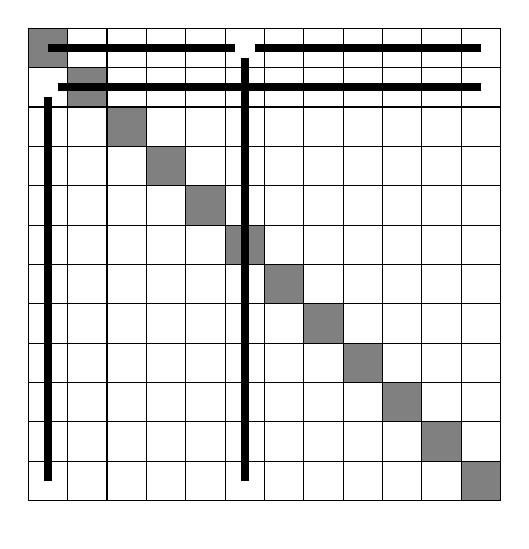
\begin{tikzpicture}[scale = 0.5]
    \path (0,-0.5) -- (0,6.5);
    \foreach \i in {0,...,11} { \fill[gray] (\i, 12-\i) rectangle (\i + 1, 11 - \i); }
    \draw (0,0) grid (12,12);
    \node (R1) at (5.5, 11.5) {\Large\symrook};
    \node (R2) at (0.5, 10.5) {\Large\symrook};
    \draw[line width = 3]
      (0.5,11.5) -- (R1) -- (11.5,11.5)
      (R1) -- (5.5,0.5)
    ;
    \draw[line width = 3]
      (R2) -- (11.5,10.5)
      (R2) -- (0.5,0.5)
    ;
  \end{tikzpicture}
  ~~
  
\begin{tikzpicture}[scale = 0.5]
    \path (0,-0.5) -- (0,6.5);
    \foreach \i in {1,...,3} { \fill[gray] (\i, 11-\i) rectangle (\i + 1, 10 - \i); }
    \foreach \i in {4,...,9} { \fill[gray] (\i, 10-\i) rectangle (\i + 1, 9 - \i); }
    \draw (0,0) grid (10,10);
  \end{tikzpicture}
  \caption[The derived board for a prefix of a derangement.]{An example of a prefix $\alpha = (6, 1)$, and the board that results
  from deleting the first $\ell = 2$ rows and columns $6$ and $1$.
  The derived complementary board of $B$ from $\alpha$ is
  $B^c_\alpha = \{(1,2), (2,3), (3,4), (5,5), \dots, (10,10)\}$.}
\label{fig:derangementPrefix}
\end{figure}
